% !TeX spellcheck = it_IT
\section{Progettazione concettuale}

\begin{figure}
    \centering
    \caption{Diagramma ER - progettazione concettuale}
    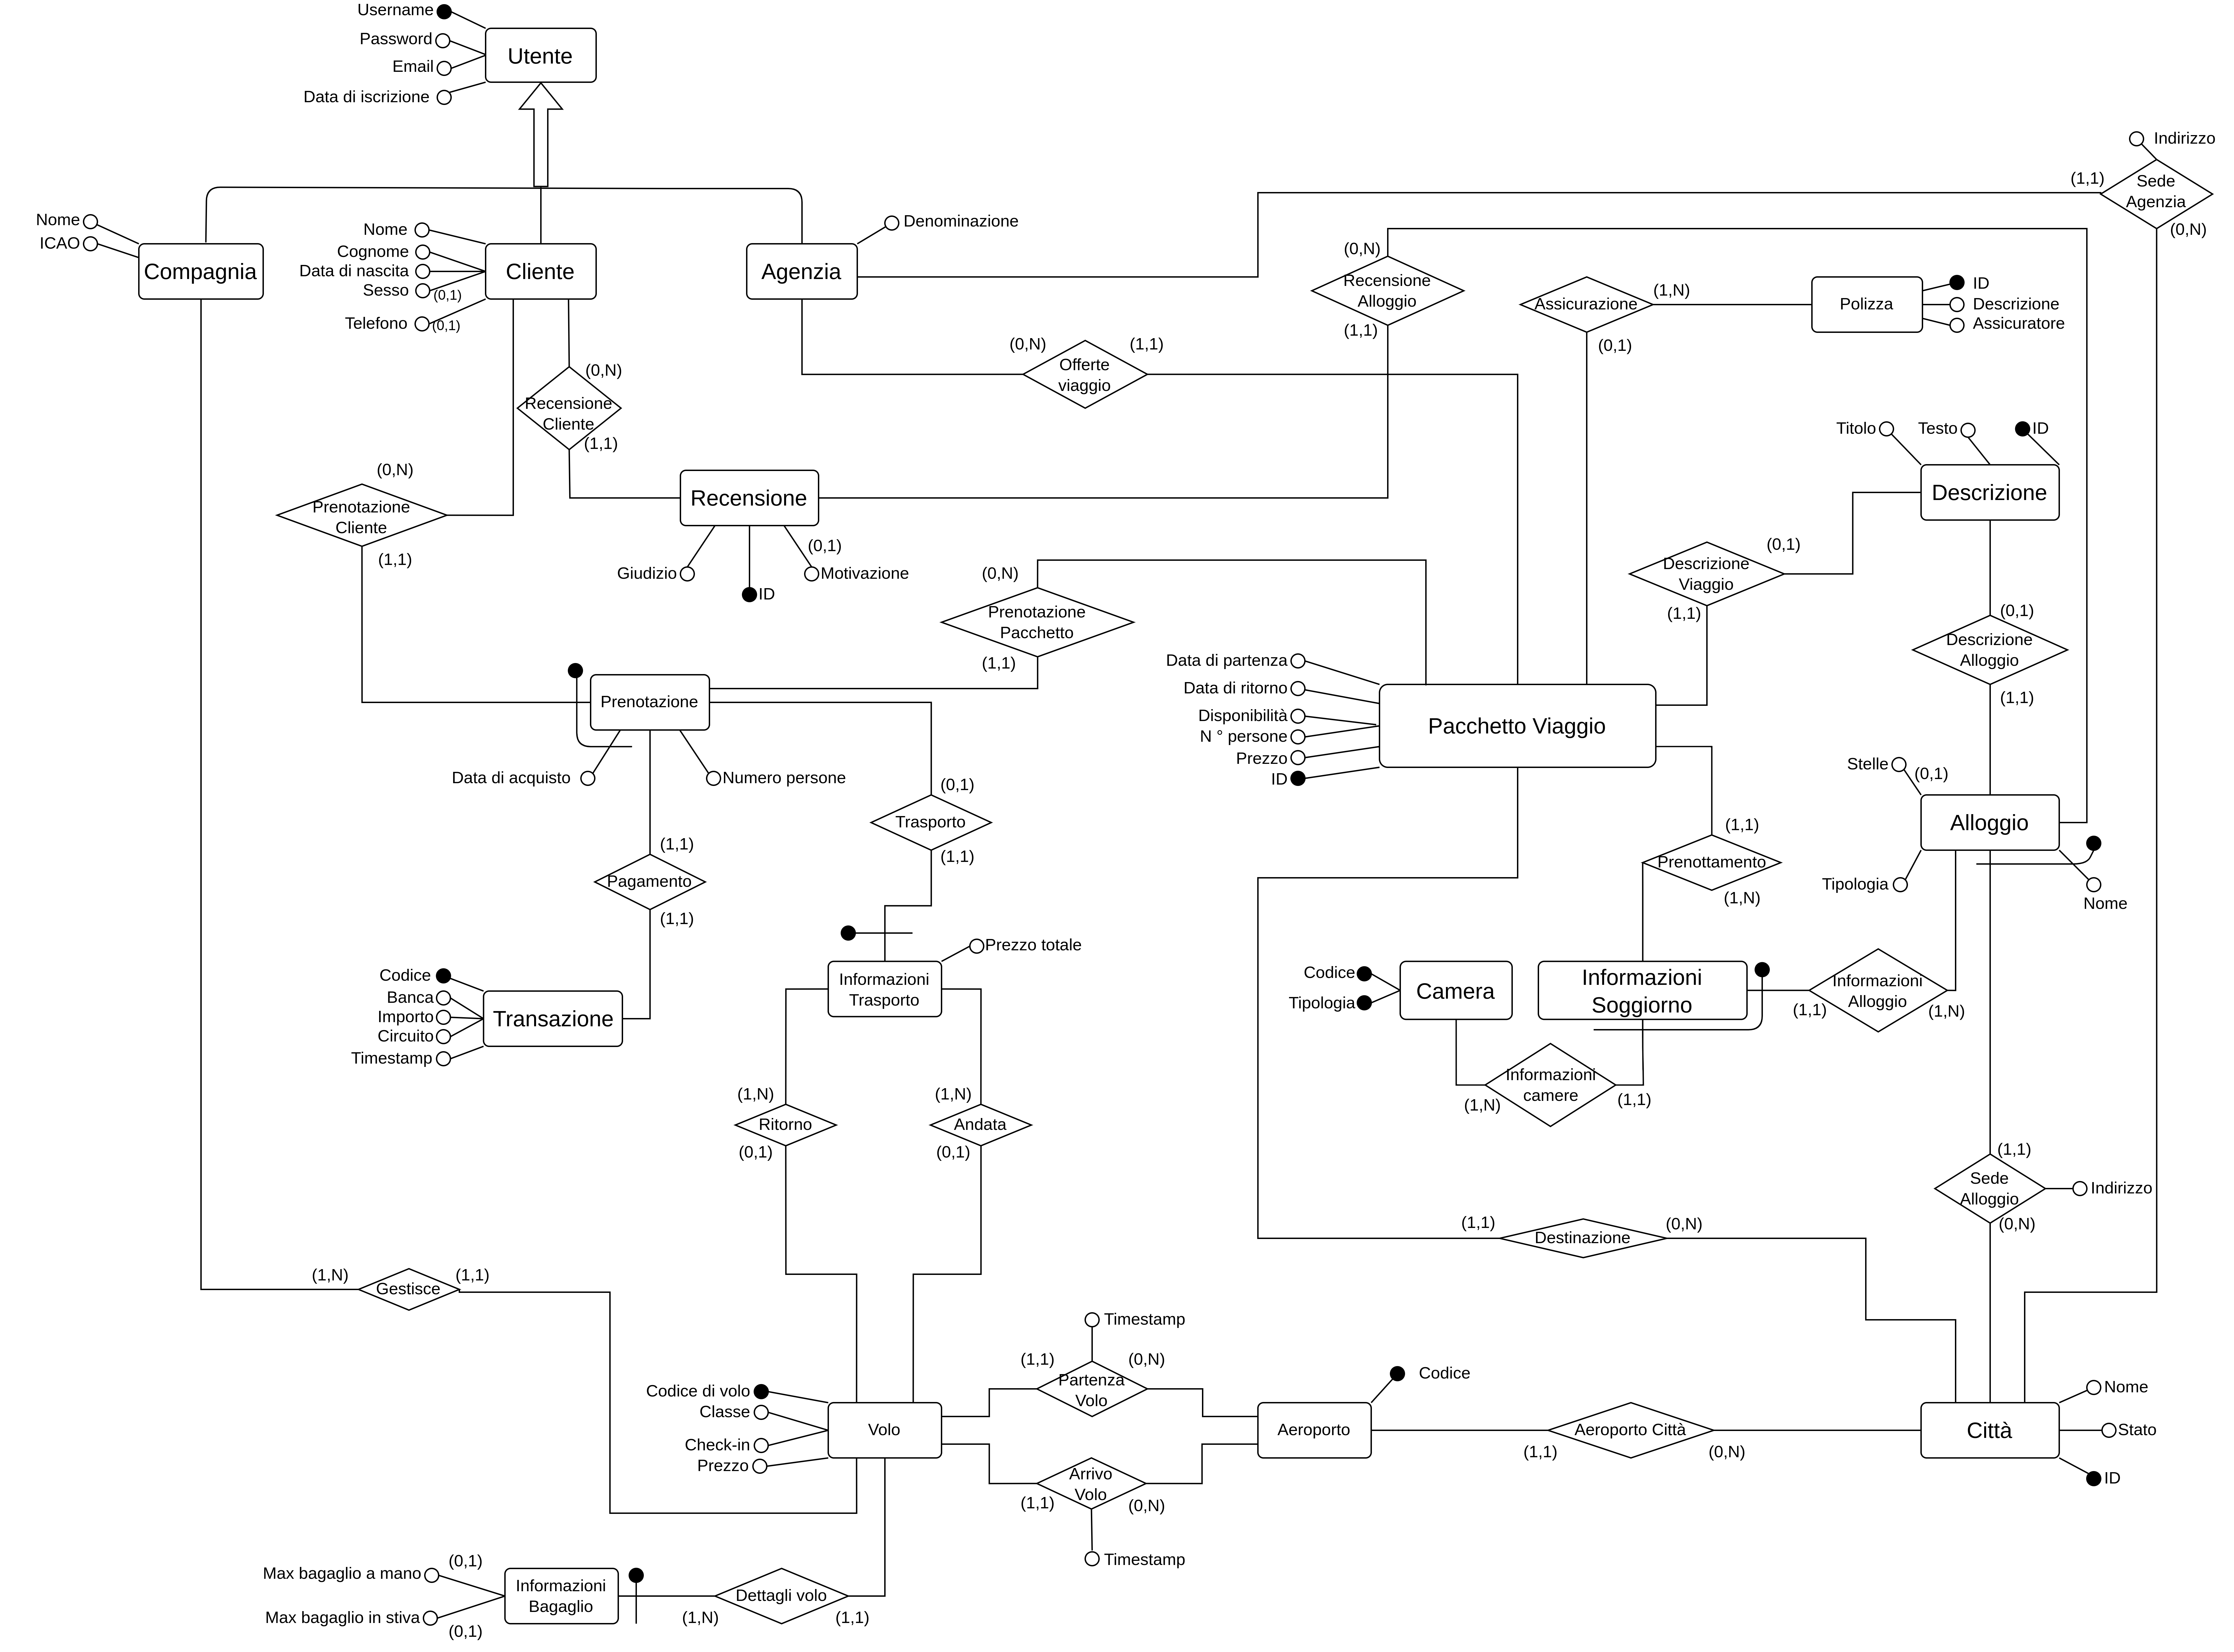
\includegraphics[width=0.85\textwidth]{assets/ER_concettuale.png}
    \label{fig:er_concettuale}
\end{figure}

\subsection{Tabelle delle entità}
\begin{center}
    \begin{tabularx}{\textwidth}{p{0.2\textwidth} X p{0.3\textwidth}}
        \caption{Tabella delle entità}\\\toprule\endfirsthead
        \toprule\endhead
        \midrule\multicolumn{3}{r}{\itshape Continua nella pagina successiva}\\\midrule\endfoot
        \bottomrule\endlastfoot
        %
        %
        \textbf{Entità} & \textbf{Descrizione dell'operazione} & \textbf{N°. operazioni}
        \\
        && (\textbf{operazioni/tempo})\footnote{Riportiamo misure di tempo: \textbf{dd} = giorni, \textbf{mm} = mesi \& \textbf{yy} = anni.}
        \\\midrule
        \emph{Inserimento pacchetto} & Inserimento di un pacchetto da parte di una agenzia & 10 o/dd
        \\
    \end{tabularx}
\end{center}

\subsection{Tabelle delle relazioni}

\subsection{Regole Aziendali}
Di seguito riportiamo i vincoli non esprimibili attraverso il diagramma ER.
\subsubsection{Vincoli di integrità}
\subsubsection{Derivazioni}